\section{Background}
\label{sec:background}
Recent shifts to microservice architectures and the resulting servicemesh have prioritized development and deployment efficency over performance.
Microservices deployed on a servicemesh (i.e. Istio~\cite{istio}) use proxies which are co-located with microservices.
These proxies intercept and control networking communication between services.
The proxies are relatively lightweight, but use the networking stack for communication with the co-located service (Figure-\ref{fig:no_kmap}).
This is done to preserve a common interface for services-- the networking stack.
Istio uses Envoy~\cite{envoy} which is the tool we focus on here for \sysname.

\subsection{Envoy}
Via a modified routing table, Envoy intercepts the incoming connections and relays those to the local services (see Figure-\ref{fig:envoy}). 
The inbound and outbound handlers handle upstream and downstream requests. 
All the routed requests are passed around using local sockets (e.g. Unix Domain Sockets). 
When a service is using Envoy, it only needs to specify a local address and a port number that it will be using, and Envoy contacts the local service through that address. 

\begin{figure*}[!htb]
    \begin{minipage}{\textwidth}
        \centering
        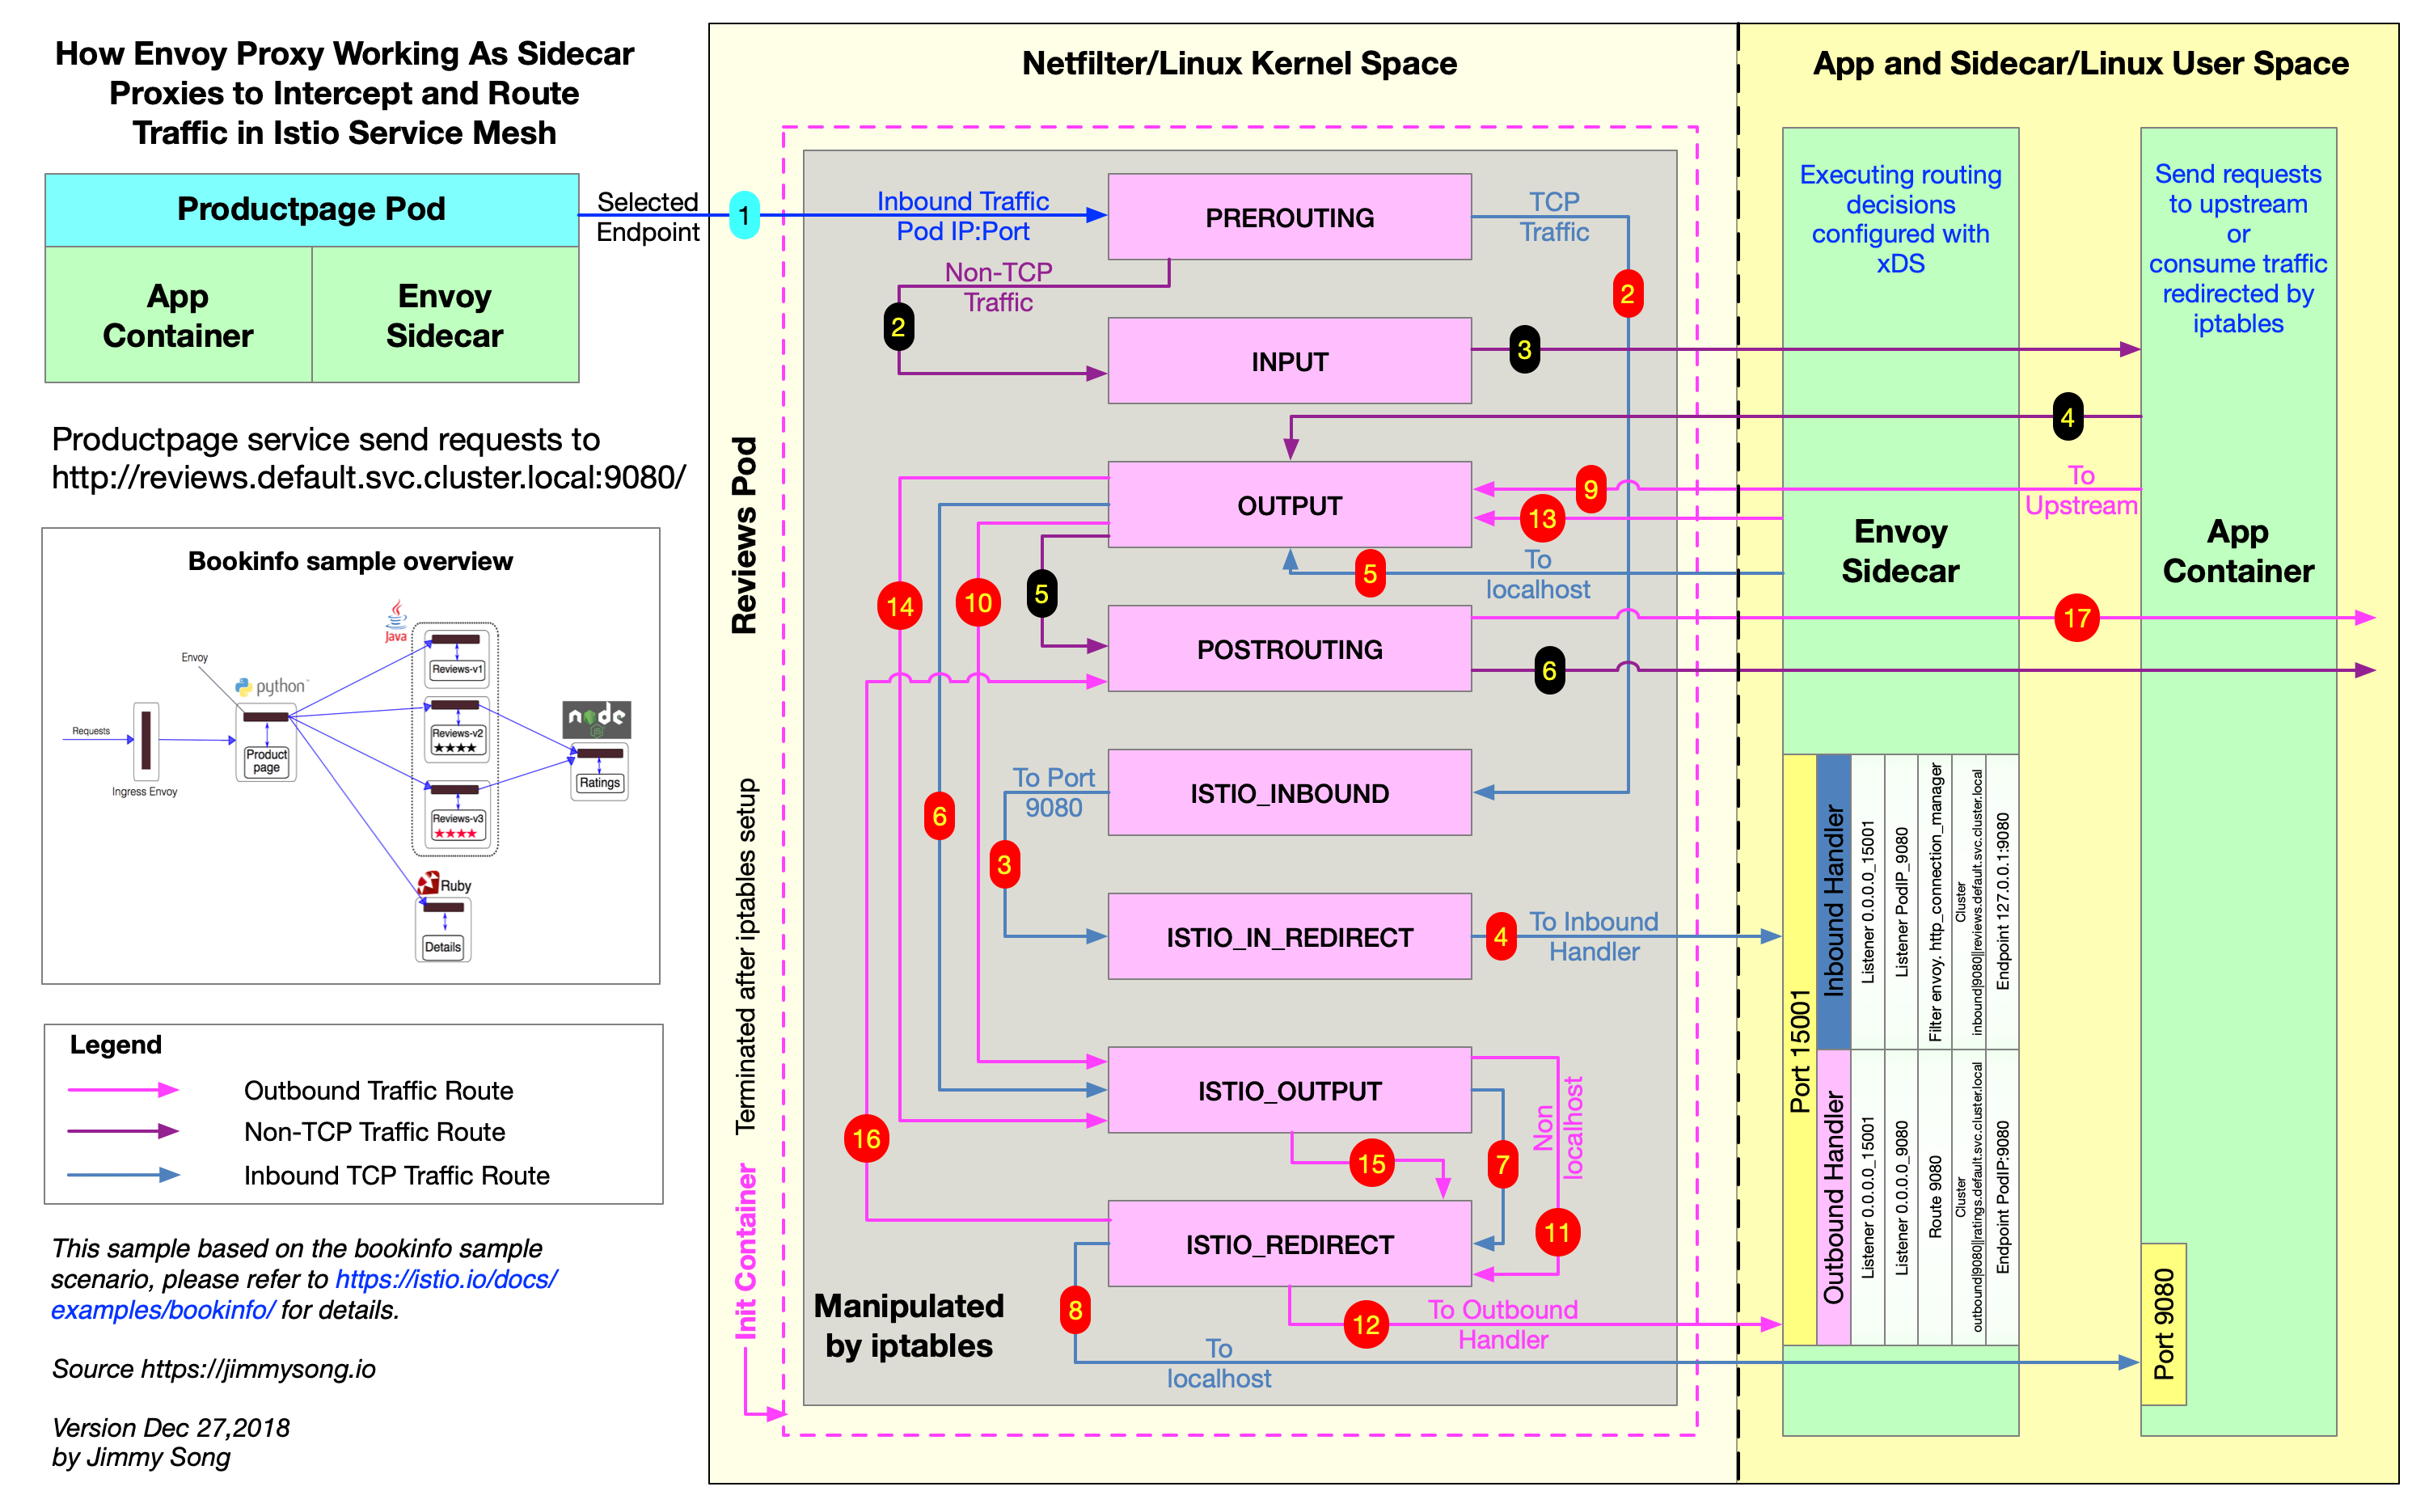
\includegraphics[keepaspectratio=true,width=7in]{figures/background/envoy.png}
        \caption{Envoy Network Stack~\cite{envoy_image}}
        \label{fig:envoy}
    \end{minipage}%
\end{figure*}

\begin{figure*}[!htb]
    \begin{minipage}{0.5\textwidth}
        \centering
        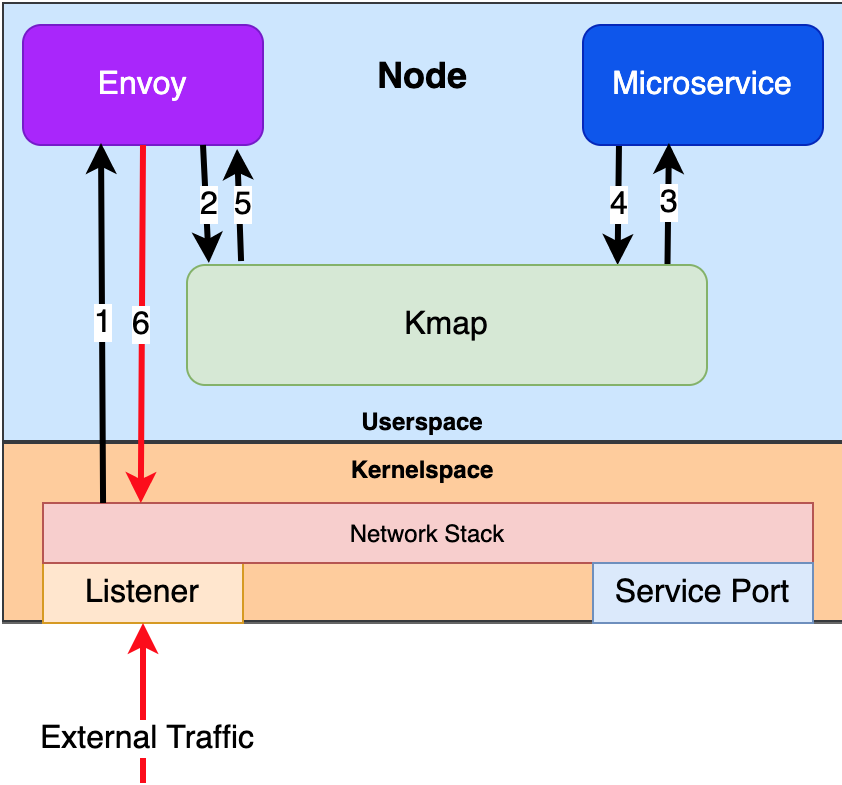
\includegraphics[keepaspectratio=true,width=3in]{figures/design/kmap.png}
        \caption{Kmap}
        \label{fig:kmap}
    \end{minipage}%
    \begin{minipage}{0.5\textwidth}
        \centering
        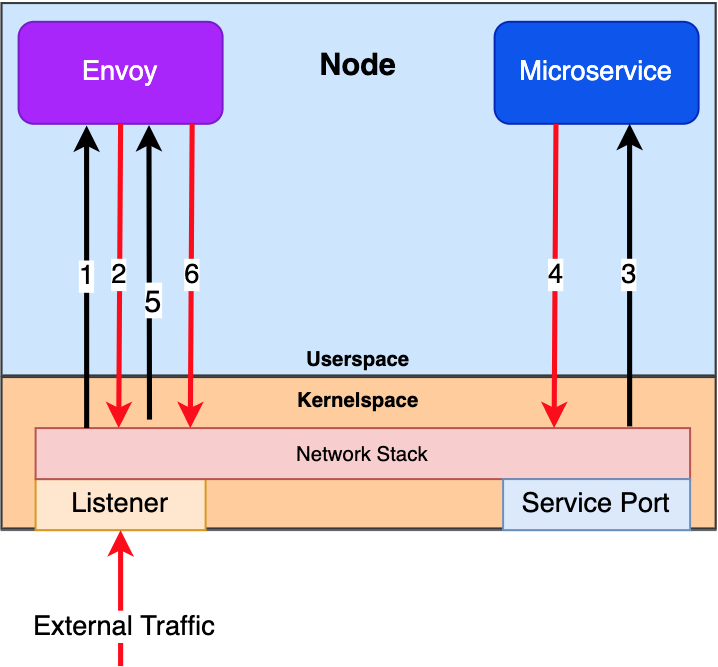
\includegraphics[keepaspectratio=true,width=3in]{figures/design/no_kmap.png}
        \caption{No Kmap Envoy Network Stack}
        \label{fig:no_kmap}
    \end{minipage}%
\end{figure*}

%
%\subsection{Linux Network Stack}
%To provide better encapsulation of data packets and avoid costly copies, Linux kernel handles packet relay between different network layers via a struct known as \texttt{sk\_buff} (short for socket buffers). Each \texttt{sk\_buff} struct keeps track of pointers to start and end of different frames and, instead of copying the whole network packet between layers, shares the \texttt{sk\_buff} for faster processing of network packets.
%
%For Unix domain sockets, however, the network stack need not be invoked. The OS often realizes that the sockets are for local purposes only and will skip some of the

%\begin{figure}[!htb]
%    \begin{minipage}{0.5\textwidth}
%        \centering
%        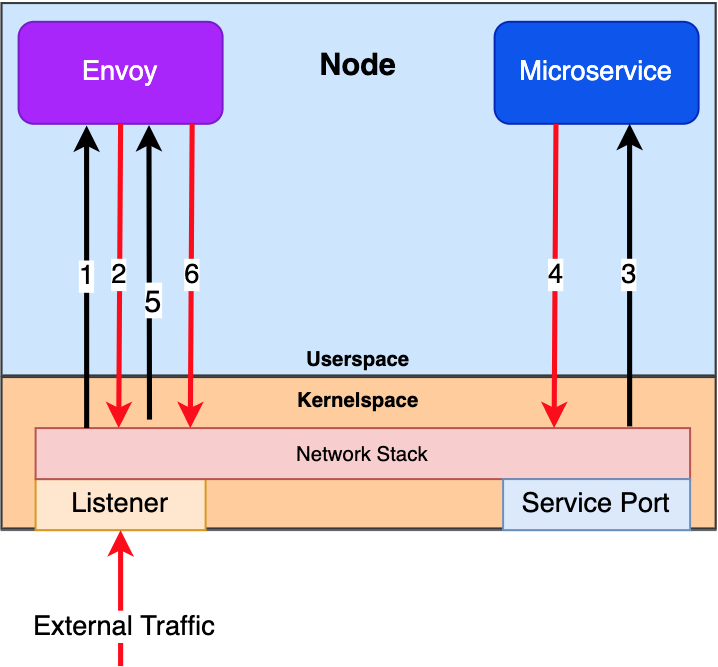
\includegraphics[keepaspectratio=true,width=3in]{figures/design/no_kmap.png}
%        \caption{No Kmap Envoy Network Stack}
%        \label{fig:no_kmap}
%    \end{minipage}%
%\end{figure}

